\documentclass{tmr}

\usepackage{mflogo}

%include lhs2TeX.fmt
%include lhs2TeX.sty
%include polycode.fmt

\newcommand{\ToDo}[1]{\textbf{ToDo}{#1}}

\title{High Performance Haskell with MPI}
\author{Bernie Pope\email{bjpope@unimelb.edu.au}}
\author{Dmitry Astapov\email{dastapov@gmail.com}}

\newcommand{\Todo}[1]{{\textbf{Todo: #1}}}

\begin{document}

\begin{introduction} 
What is MPI, what is haskell-mpi, how can you use it for writing multi-node programs in Haskell or interoperate with other languages
\end{introduction}

\section{Distributed-memory parallelism and MPI}

The World's largest supercomputers now feature hundreds of thousands of CPU cores, and mega-core machines
are just around the corner.\footnote{As one example, the Lawrence Livermore National Laboratory (LLNL) 
is currently
preparing to install Sequoia, a 1.25 million core IBM BlueGene/Q: \url{www.llnl.gov}} There are many technical
challenges to building such behemoths, not the least of which is
the CPU-to-memory bottleneck. Shared memory parallel computers --- which now dominate consumer-grade
systems --- provide the convenient abstraction that every processor has equivalent access to all memory,
even though the underlying connections between processors and memory are typically non-uniform.
Unfortunately (and unsurprisingly) it is difficult to scale this abstraction in a
cost-effective way to the supercomputing level. A quick glance at the Top 500 list of supercomputers reveals
no significant large-scale shared-memory systems.\footnote{\url{www.top500.org}}
Instead we see that practically all the listed supercomputers are based on
disributed-memory parallelism. These machines are built from many independent computers (called nodes),
each with their own processors, memory and operating system, connected by one or more high-speed networks.
The nodes themselves are often smaller multi-core shared-memory computers, nevertheless
the macro architecture is distributed.

Distributed-memory parallelism does not really solve the CPU-to-memory bottleneck (over the whole machine),
afterall, sharing data between nodes over a network is a relatively costly operation.
Instead it forces programmers to
address the non-uniformity head on, which typically means adopting an explicitly distributed style of
parallel programming,\footnote{There have been several attempts to provide a shared-memory like abstraction
on top of distributed parallel machines, such as Unified Parallel C, but automated load balancing remains
an open problem.} and often requires new algorithms to be devised.

The Message Passing Interface (MPI) is a standardised parallel programming
system which is designed to help programmers write large-scale
distributed-parallel programs~\cite{mpi-report}. As the name suggests,
MPI is based on independent computing processes which collaborate by passing
messages amongst themselves.  Given the bias in supercomputing to scientific applications,
it is not too surprising to find that the MPI standard defines APIs for Fortran, C
and C++. There are numerous APIs provided for other languages,
usually by making foreign calls to the C interface --- that is precisely the way
Haskell-MPI works.

Haskell-MPI provides two basic interfaces:
\begin{enumerate}
 \item A simple high-level interface designed to make
it convenient to use arbitrary serialisable data structures as messages.
 \item A more intricate lower-level interface designed to reduce
performance overheads when using array-like data structures as messages.
\end{enumerate}
Despite the different focus of the interfaces, they are both quite similar in
spirit to the underlying C API. This means it is quite easy to port code
from one of the standard interfaces to Haskell, but is also means
that (unfortunately) Haskell-MPI inherits some of the type unsafety of
MPI's design, and is rather imperative in attitude.

The purpose of this article is to introduce you to some of the basic concepts
of distributed parallel programming with Haskell-MPI. We begin by introducing
the technique of computing definite integrals by the Trapezoid Method.
This gives rise to an easy-to-parallelise algorithm which will serve as the
basis of programming examples in later sections.

%\section{Very short intro to MPI and haskell-mpi and outlining the motivation}
%What is MPI? If you ever tried to make processes running on separate
%computers talk to each other, chances are that you already came across
%the MPI or invented parts of it. 

%Even though MPI has been standartized only aroung 1995\footnote{Full
%  formal definition of protocol, its semantics and reference
%  implementation could be found in \cite{mpi-report}}, it has become
%de-facto standart in programming on architecures with distributed
%memory (``clusters'' or ``parallel computers''). It tries to prove a
%language-independent communications means that would allow users to
%pass around ``messages'' (hence the name, ``Message Passing
%Interface''). We have it on a good authority that MPI is still widely
%used today, even though there are numerous alternatives for
%inter-process communication. This article would focus on haskell-mpi,
%not trying to provide any sort of comparison with possible
%alternatives, as authors believe that any choice like this should
%ultimately be made in context of the specific task at hand.

%So what is, then, haskell-mpi? It is a package of low- and high-level bindings
%to C MPI library that allows Haskell programmers to call upon the
%powers of MPI with ease. 

%What would be the most (stereo)typical use case for haskell-mpi?
%Suppose that you have a task which easily lends itself to subdivision
%into a number of independent subtasks. In this day and age, when
%having multiple networked computers in vicinity is more of a rule than
%an exception, it is only natural to try and execute all the subtasks
%on different machines in parallel and then combine their results.

\section{Computing definite integrals using the Trapezoid Method}

\begin{figure*}[t]
\centering
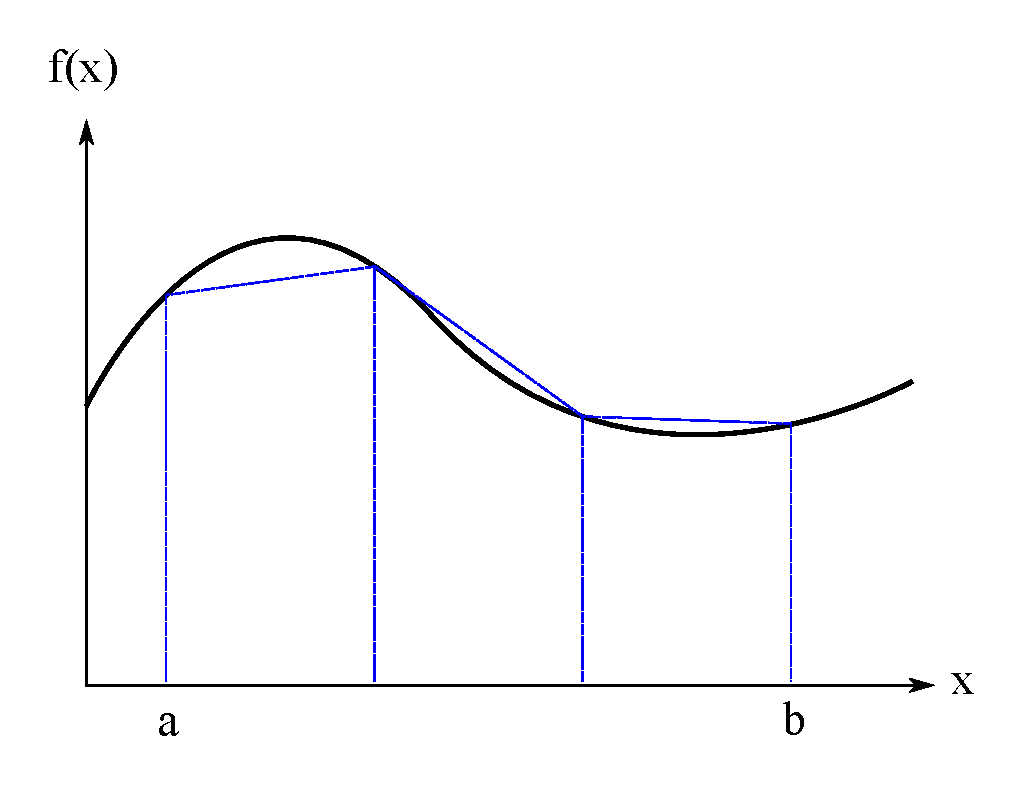
\includegraphics[width=8cm]{integral_diag.pdf}
\caption{Approximating $\int_{x=a}^{b} f(x)$ by summing the area of three trapezoids. }
\end{figure*}

Consider very simple numerical integration code, which tries to
compute $\int_{x=a}^{b} f(x)$ using $n$ steps:
% ./code/Trapezoid.hs
\begin{listing}
\begin{Verbatim}
module Main where

import System (getArgs)

main :: IO ()
main = do
  aStr:bStr:nStr:_ <- getArgs
  let [a,b] = map read [aStr,bStr]
      n = read nStr
      h = (b - a) / fromIntegral n
      integral = trapezoid f a b n h
  print integral 

-- Integrate 'f' on interval [a,b] using 'n' steps of size 'h'
trapezoid :: (Double -> Double) -> Double -> Double -> Int -> Double -> Double
trapezoid f a b n h =
  h * sum (endPoints:internals)
  where
  endPoints = (f a + f b) / 2
  internals = map f $ take (n - 1) $ iterate (+h) (a + h)

f :: Double -> Double
-- f x = 4 / (1 + x * x)
-- f = cos
f = const 1
\end{Verbatim}
\end{listing}

After splitting interval into arbitrary number of parts you could
integrate them separately and them sum the results. In fact, very
simple modification is required to make this code use all available
cores in single multi-cored machine:
\begin{Verbatim}
TODO: put threaded code here
\end{Verbatim}

\ToDo Actually, I am having problems making our naive aproach to
paralellize without explicitly introducing chunking or threads :(

But what if you want to do that on more that one box to utilise even
bigger number of cores? You would have, at the very least, tell the
processes on each node which part of the task they would work on, and
later on you would have to gather and combines results from them.

This could be done manually, but if you want to run the program
repeatedly, or if your interprocess communications are even slightly
more complex, you would need some means of communication between
processes. In pseudo-code, this would look like this:

\begin{compactitem}
\item find number of available nodes
\item split interval between them
\item tell each node the interval it would work on
\item perform work (integration) on each node and send result to master node
\item collect results from nodes
\item sum them up
\end{compactitem}

\ToDo: ideas for further sections: show how easy it would be to extend this to ``find number of nodes AND number of cores on them, split work according to power of node''


\section{Introducing haskell-mpi}

Good news! Pseudo-code from the previous section could be directly translated into haskell code:

\begin{Verbatim}
module Main where

import Control.Parallel.MPI.Simple
import System (getArgs)

main :: IO ()
-- TODO: maybe explicit commRank/commSize would be better here? Or
-- even further below, right besides the ``if'' ?
main = mpiWorld $ \numRanks rank -> do
  aStr:bStr:nStr:_ <- getArgs
  let [a,b] = map read [aStr,bStr]
      n = read nStr
      h = (b - a) / fromIntegral n
      localN = n `div` fromIntegral numRanks
      localA = a + fromIntegral rank * fromIntegral localN * h
      localB = localA + fromIntegral localN * h
      integral = trapezoid f localA localB localN h
  if rank == 0
     then print . sum =<< gatherRecv commWorld 0 integral
     else gatherSend commWorld 0 integral

trapezoid :: (Double -> Double) -> Double -> Double -> Int -> Double -> Double
trapezoid f a b n h =
  h * sum (endPoints:internals)
  where
  endPoints = (f a + f b) / 2
  internals = map f $ take (n - 1) $ iterate (+h) (a + h)

f :: Double -> Double
f x = 4 / (1 + x * x)
\end{Verbatim}
%% $ - for naive auctex mode that thiks that math mode somehow escapes
%% from Verbatim and rules over the rest of the text. AuCTeX, you are wrong!

Here, \verb|commWorld| is a ``code name'' for the default group of processes
(``communicator'' in MPI terminology), which includes all the
processes participating in this particular run. Processes in the group
are numbered starting with zero. We've implemented
``many-to-one'' communication pattern, with process number 0
collecting data sent by all other processes (using \verb|gatherSend|)
and putting them into a list.

It might seem strange at first that processes do no exchange any
messages to determine how to divide the work among themselves. That is
because an established practice in MPI world is to run the same binary
on all computers (``nodes'') participating in the run, to reduce
development and deployment efforts. This way, if some run-time
parameters could be deduced solely from process number (``rank'') and
the information available to all processes at startup, it would not
require any additional message passing.

Thus, code that uses MPI usualy features a substantial pieces of code,
which, while present in all binaries, are actually executed only in
some of the running copies. While programming with MPI in C, care must
be taken to avoid allocations/computations in processes that would not
actually use the appropriate data, and to avoid referencing/using
uninitialized data. Haskell, with its lazy evaluation and automatic
memory management, allows to significantly reduce amount of mental
energy required to get everything right. If computations are pure,
they simply would not be executed in the processes that don't use
them, withough requiring any explicit ``housekeeping'' code.

\ToDo it would've been nice to have something like that in our
example, but ... well ...

\ToDo quickly introduce ``communicators'' and ``ranks'' here, refer
readers to MPI docs and books for further reading (in footnote). Not
sure it is needed here anymore.

\ToDo Would this be relevant anywhere at all? Messages could be sent from process to process or
dispatched to/from all process in a group, called in MPI terminology ``communicator''.


\section{Does this really speeds things up?}

In order to compile and run our sample integration code, you have to
have \verb|haskell-mpi| package installed\footnote{Please refer to
  \ref{appendix-A}{Appendix A} for installation and running help}. After that,
simple \verb|ghc --make -O2 <file>.hs| should be sufficient to produce
a working MPI-enabled binary.

Even if you don't have several networked computers, you could still
run several processes on the same box, which actually makes sense if
you have multiple CPU cores. OpenMPI would do this by default if you
haven't configured your ``computing network'' topology. Try running
\verb|mpirun -n <N> ./ToDoNameHere ToDoArgsHere|, where \verb|N| is
from 2 up to the number of cores you have.

\ToDo would it run with 1 process?

You should be able to observe almost linear speed up. We were able to
test this code on quite large computing cluster and got the following
numbers\footnote{runtimes from N tries, averaged}:

\ToDo: measurement results here, table and graph.

As you can see (describe something less obvious that could be derived
from the graph, for example that for large N computation takes less
time than transmission of the results).

Mention serialization. In our examples result of the computation was a
simple double and \verb|cereal| already knows how to serialize all
primitive types, and tuples, lists and arrays of them. For
user-defined types it is necessary to provide instances of typeclass
\verb|Serialize|, but they are quite trivial (ref to McPhd ``patch''
here?)

\ToDo: we could also do this: We even took some less-trivial haskell
code (McPhd) and applied the same approach to parallelize it (href to
patch on git-hub) and here is what we've got: another table and graph.

\section{I'm hooked. What else could haskell-mpi do?}


You could use it to combine haskell and C code. Here is how: (separate sub-section on this?)
\subsection{Interacting with C}
\begin{Verbatim}
#include <mpi.h>
#include <stdio.h>
#include <stdlib.h>
#include <math.h>

double f(double);
double trapezoid(double, double, int, double);

int main(int argc, char **argv) {
   double a, b, h, local_a, local_b, integral, sum = 0;
   double *results = NULL;
   int n, local_n, rank, num_ranks;

   MPI_Init(&argc, &argv);
   MPI_Comm_size(MPI_COMM_WORLD, &num_ranks);
   MPI_Comm_rank(MPI_COMM_WORLD, &rank);

   a = atof(argv[1]);
   b = atof(argv[2]);
   n = atoi(argv[3]);

   h = (b - a) / n;
   local_n = n / num_ranks;
   local_a = a + rank * local_n * h;
   local_b = local_a + local_n * h;
   integral = trapezoid(local_a, local_b, local_n, h);

   if (rank == 0) {
      results = (double *) malloc(num_ranks * sizeof(double));
   }

   MPI_Gather(&integral, 1, MPI_DOUBLE, results, 1, MPI_DOUBLE, 0, MPI_COMM_WORLD);

   if (rank == 0) {
      for (int i = 0; i < num_ranks; i++) {
         sum += results[i];
      }
      printf("%lf\n", sum);
   }
   MPI_Finalize();
}

double trapezoid(double a, double b, int n, double h) {
   double result;
   double x = a;
   result = (f(a) + f(b)) / 2.0;
   for (int i = 1; i < n; i++) {
      x = x + h;
      result += f(x);
   }
   return result * h;
}

double f(double x) {
   return 4.0 / (1 + x * x);
}
\end{Verbatim}


Or you can you is to implement less trivial communication patterns (allreduce example or something more complex?)


\section{Conclusion, further reading, next steps, ...}

\ToDo mention somewhere bundled example and tests that could provide inspiration :)

Full \verb|haskell-mpi| sources\footnote{github, cabal source
  haskell-mpi} also contain a comprehensive testsuite and a set of
examples, which demonstate the use of all of the supported functions.

\ToDo mention Well-Typed

\section{Appendix A: Installation and tested MPI implementations}
\label{appendix-A}
We tested the code on MPICH 1.2.x and 1.4.x, OpenMPI x.y.z. Amount of implementation-specific code is minimal and there is a good chance that all the other MPI implementations would be supported out of the box.

To install, try ``cabal install haskell-mpi''. If that fails to find MPI include/library files in system-wide directories, try ...
\ToDo provide installation cmdline

\bibliography{haskell-mpi}

\end{document}
